\documentclass[handout,compress]{beamer}

\usetheme[block=fill]{metropolis}

\usepackage{graphicx} % Allows including images
\usepackage{amsmath,amsfonts,amsthm,amssymb}
\usepackage{color}
\usepackage{xcolor,cancel}
%\setitemize{label=\usebeamerfont*{itemize item}%
%	\usebeamercolor[fg]{itemize item}
%	\usebeamertemplate{itemize item}}
\definecolor{mDarkBrown}{HTML}{604c38}
\definecolor{mDarkTeal}{HTML}{23373b}
\definecolor{mLightBrown}{HTML}{EB811B}
\definecolor{mMediumBrown}{HTML}{C87A2F}
\definecolor{mygreen}{HTML}{98C2B9}
\definecolor{myyellow}{HTML}{DFD79C}
\definecolor{myblue}{HTML}{8CA7CC}
\definecolor{kern}{HTML}{8CC2B7}

\usepackage{float}
\usepackage{framed}
\usepackage{epsfig}
\usepackage{graphicx}
\usepackage{subcaption}
\usepackage{ulem}
\usepackage{hhline}
\usepackage{multirow}
\usepackage{comment}   
\usepackage{bbm}
\usepackage{tikz}   
\usepackage{ulem}
\def\Put(#1,#2)#3{\leavevmode\makebox(0,0){\put(#1,#2){#3}}}
\newcommand*\mystrut[1]{\vrule width0pt height0pt depth#1\relax}
\newcommand{\eqdef}{\mathbin{\stackrel{\rm def}{=}}}


\newcommand{\bs}[1]{\boldsymbol{#1}}
\newcommand{\bv}[1]{\mathbf{#1}}
\newcommand{\R}{\mathbb{R}}
\newcommand{\E}{\mathbb{E}}

\DeclareMathOperator*{\argmin}{arg\,min}
\DeclareMathOperator*{\argmax}{arg\,max}
\DeclareMathOperator{\nnz}{nnz}
\DeclareMathOperator{\Var}{Var}
\DeclareMathOperator{\sinc}{sinc}
\DeclareMathOperator{\mv}{mv}
\DeclareMathOperator{\sgn}{sgn}
\DeclareMathOperator{\step}{step}
\DeclareMathOperator{\gap}{gap}
\DeclareMathOperator{\poly}{poly}
\DeclareMathOperator{\tr}{tr}
\DeclareMathOperator{\orth}{orth}
\newcommand{\norm}[1]{\|#1\|}
\captionsetup[subfigure]{labelformat=empty}
\captionsetup[figure]{labelformat=empty}
\DeclareMathOperator*{\lmin}{\lambda_{min}}
\DeclareMathOperator*{\lmax}{\lambda_{max}}

\newcommand{\specialcell}[2][c]{%
  \begin{tabular}[#1]{@{}c@{}}#2\end{tabular}}
\newcommand{\specialcellleft}[2][c]{%
\begin{tabular}[#1]{@{}l@{}}#2\end{tabular}
}

\usepackage{tabstackengine}
\stackMath


%----------------------------------------------------------------------------------------
%	TITLE PAGE
%----------------------------------------------------------------------------------------

\title{CS-UY 4563: Lecture 7 \\ The Bayesian Perspective cont., Linear Classifiers}
\author{NYU Tandon School of Engineering, Prof. Christopher Musco}
\date{}

\begin{document}

\begin{frame}
	\titlepage 
\end{frame}

\metroset{titleformat=smallcaps}

\begin{comment}
\end{comment}

\begin{frame}
	\frametitle{probabilistic modeling}
		In a \emph{Bayesian} or \emph{Probabilistic} approach to machine learning we always start by conjecturing a
		\begin{center}
			\textbf{probabilistic model}
		\end{center}
		that plausibly could have generated our data.
		
		\begin{itemize}
			\item The model guides how we make predictions.
			\item The model typically has unknown parameters $\vec{\theta}$ and we try to find the most reasonable parameters based on observed data (more on this later in lecture).
		\end{itemize}
\end{frame}

\begin{frame}
	\frametitle{probabilistic modeling}
	\textbf{Exercise:} With a partner, come up with a probabilistic model for \emph{any one} of the following data sets $(x_1, y_1), \ldots, (x_n,y_n)$.
	\begin{enumerate}
		\item For $n$ \textbf{people}: each $x_i \in \{0,1\}$ with zero indicating \emph{male}, one indicating \emph{female}. Each $y_i$ is the height of the person in inches. 
		\item For $n$ \textbf{NYC apartments}: each $x_i$ is the size of the apartment in square feet. Each $y_i$ is the monthly rent in dollars. 
		\item For $n$ \textbf{students}: each $x_i \in \{Fresh.,Soph.,Jun.,Sen.\}$ indicating class year. Each $y_1 \in \{0,1\}$ with zero indicating the student has not taken machine learning, one indicating they have.
	\end{enumerate}
	
	\vspace{-.5em}
	\begin{center}
		\alert{Record any unknown parameters of your model. What would be a guess for their values? How would you confirm or refine this guess using data?}
	\end{center}
\end{frame}

\begin{frame}[t]
	\frametitle{probabilistic modeling}
	\textbf{Dataset:} $(x_1, y_1), \ldots, (x_n,y_n)$
	
	\textbf{Description}: For $n$ \textbf{people}: each $x_i \in \{0,1\}$ with zero indicating \emph{male}, one indicating \emph{female}. Each $y_i$ is the height of the person in inches. 
	
	\textbf{Model:}
\end{frame}

\begin{frame}[t]
	\frametitle{probabilistic modeling}
	\textbf{Dataset:} $(x_1, y_1), \ldots, (x_n,y_n)$
	
	\textbf{Description}: For $n$ \textbf{NYC apartments}: each $x_i$ is the size of the apartment in square feet. Each $y_i$ is the monthly rent in dollars. 
	
	\textbf{Model:}
\end{frame}

\begin{frame}[t]
	\frametitle{probabilistic modeling}
	\textbf{Dataset:} $(x_1, y_1), \ldots, (x_n,y_n)$
	
	\textbf{Description}: For $n$ \textbf{students}: each $x_i \in \{Fresh.,Soph.,Jun.,Sen.\}$ indicating class year. Each $y_1 \in \{0,1\}$ with zero indicating the student has not taken machine learning, one indicating they have.
	
	\textbf{Model:}
\end{frame}

\begin{frame}
	\frametitle{naive bayes classifier}
	\textbf{Goal:}
	\begin{itemize}
		\item Build a probabilistic model for a binary classification problem.
		\item Estimate parameters of the model.
		\item From the model derive a classification rule for future predictions (the \alert{\textbf{Naive Bayes Classifier}}).
	\end{itemize}
\end{frame}

\begin{frame}
	\frametitle{spam prediction}
	\begin{center}
		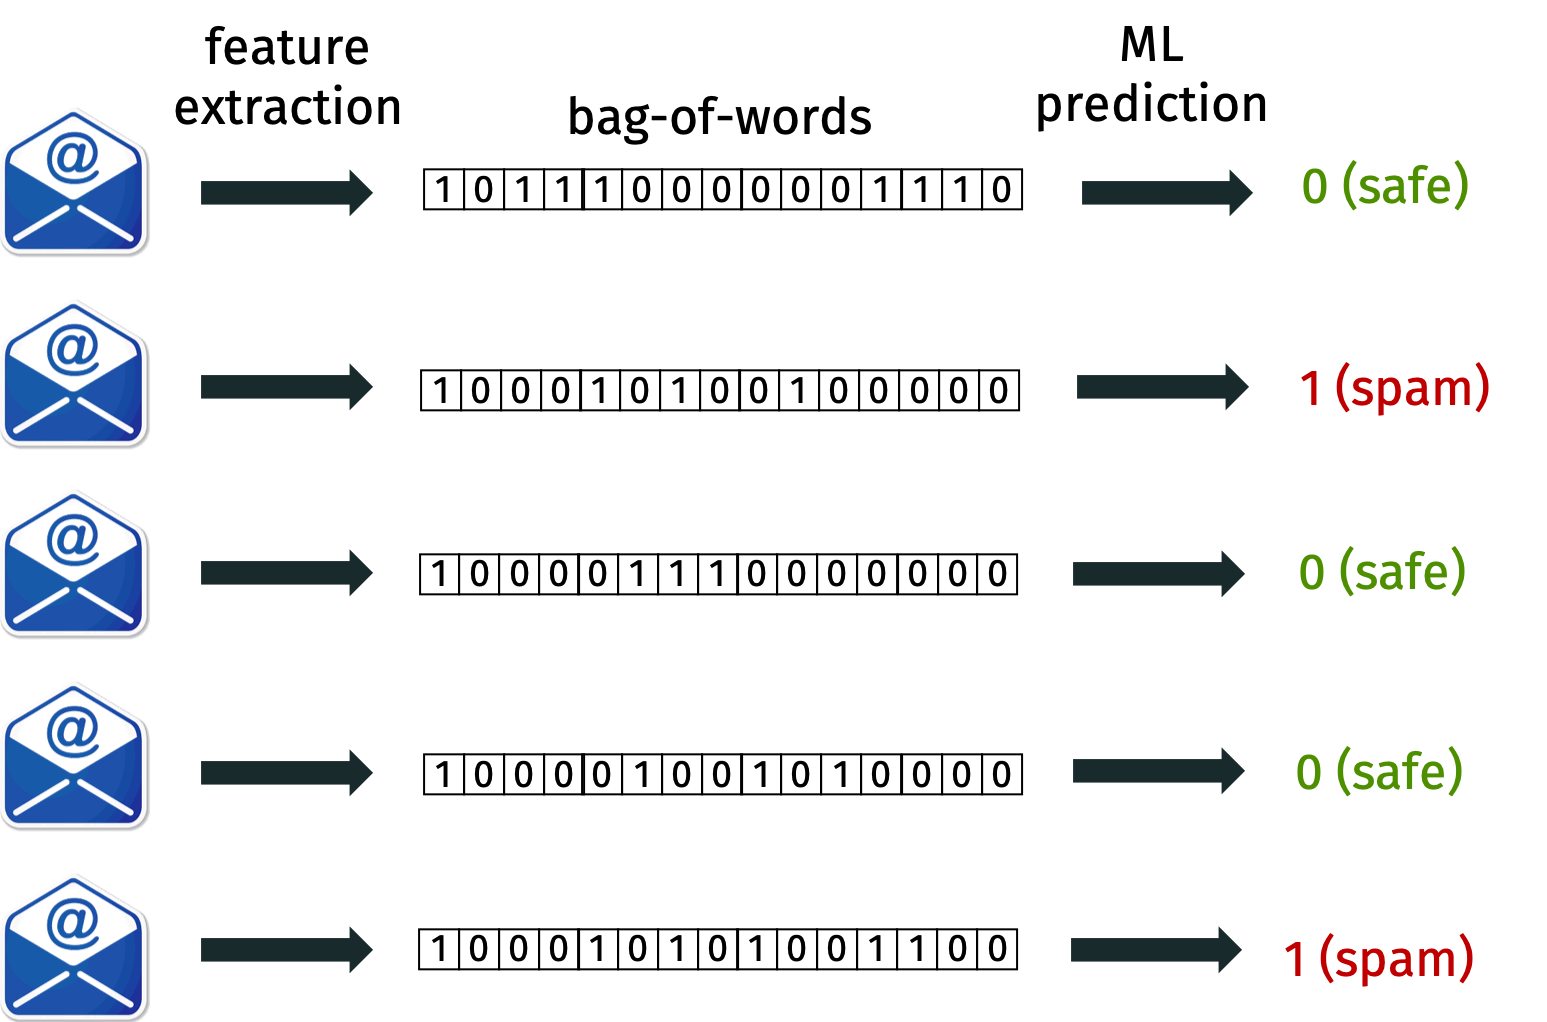
\includegraphics[width=.9\textwidth]{spam.png}
		
		\vspace{.5em}
		\textbf{Both target labels {and} data vectors are binary.}
	\end{center}
\end{frame}

\begin{frame}
	\frametitle{probabilistic model for email}
	\textbf{Probabilistic model} for  (bag-of-words, label) pair $(\bv{x},y)$:
	\begin{itemize}
		\item Set $y = 0$ with probability $p(y = 0)$, $y = 1$ with probability $p(y = 1) = 1-p(y=0)$. 
		\begin{itemize}
			\item $p(y = 0)$ is probability an email is not spam (e.g. $99\%$). 
			\item $p(y = 1)$ is probability an email is spam (e.g. $1\%$). 
		\end{itemize}
		\item If $y=0$, for each $i$, set $x_i = 1$ with prob. $p(x_i = 1 \mid y=0)$.
		\item If $y=1$, for each $i$, set $x_i = 1$ with prob. $p(x_i = 1\mid y=1)$.
	\end{itemize}

	\alert{\textbf{Unknown model parameters:}} 
	\vspace{-.5em}
	\begin{itemize}
		\item $p(y = 0), p(y = 1)$,
		\item $p(x_1 = 1 \mid y=0), \ldots, p(x_n = 1 \mid y=0)$.
		\item $p(x_1 = 1 \mid y=1), \ldots, p(x_n = 1 \mid y=1)$.
	\end{itemize} 
\begin{center}
	\textbf{How would you estimate these parameters?}
\end{center}
\end{frame}

\begin{frame}
	\frametitle{parameter estimation}
	\textbf{Reasonable way to set parameters:}
	\begin{itemize}
		\item Set $p(y = 0)$ and $p(y = 1)$ to the empirical fraction of not spam/spam emails.
		\item For each word $i$, set $p(x_i = 1 \mid y=0)$ to the empirical probability word $i$ appears in a \emph{non-spam} email.
		\item For each word $i$, set $p(x_i = 1 \mid y=1)$ to the empirical probability word $i$ appears in a \emph{spam} email.
	\end{itemize} 
	\begin{center}
		\alert{Estimating these parameters is the only ``training'' we will do.}
	\end{center}
\end{frame}

\begin{frame}[standout]
	done with modeling \\
	\alert{on to prediction}
\end{frame}

%\begin{frame}
%	\frametitle{probability review}
%	\begin{itemize}
%		\item \textbf{Probability:} p(x) -- the probability event $x$ happens.
%		\item \textbf{Joint probability:} p(x,y) -- the probability that event $x$ \emph{and} event $y$ happen. 
%		\item \textbf{Conditional Probability} $p(x \mid y)$ -- the probability $x$ happens \emph{given} that $y$ happens.
%	\end{itemize}
%
%\begin{align*}
%	p(x | y) = 
%\end{align*}
%
%\end{frame}

\begin{frame}
	\frametitle{classification rule}
	Given unlabeled input $(\bv{x},\rule{.6cm}{0.15mm})$, choose the label $y \in \{0,1\}$ which is \emph{most likely} given the data. Recall $\bv{x} = [0,0,1,\ldots, 1, 0]$. 
	
	\begin{center}
		\textbf{Classification rule:} \alert{maximum a posterior prob. (MAP) estimate.}
	\end{center}
	\textbf{Step 1. Compute:}
	\begin{itemize}
		\item $p(y=0 \mid \bv{x})$: prob. $y = 0$ given observed data vector $\bv{x}$. 
		\item $p(y=1 \mid \bv{x})$: prob. $y = 1$ given observed data vector $\bv{x}$. 
	\end{itemize}
	\textbf{Step 2. Output:} $0$ or $1$ depending on which probability is larger.
	
	\begin{center}
		$p(y=0 \mid \bv{x})$ and $p(y=1 \mid \bv{x})$ are called \textbf{\alert{posterior}} probabilities.
	\end{center}
\end{frame}

\begin{frame}
	\frametitle{evaluating the posterior}
	How to compute the posterior? \textbf{Bayes rule!}
	\begin{align}
		p(y=0 \mid \bv{x}) = \frac{p(\bv{x}\mid y=0)p(y=0)}{p(\bv{x})}
	\end{align}
	\begin{align}
	\text{posterior} = \frac{\text{likelihood}\times \text{prior}}{\text{evidence}}
	\end{align}
	\begin{itemize}
		\item \textbf{Prior:} Probability in class $0$ \emph{prior} to seeing any data.
		\item \textbf{Posterior:} Probability in class $0$ \emph{after} seeing the data.
	\end{itemize}
\end{frame}

\begin{frame}
	\frametitle{evaluating the posterior}
Goal is to determine which is larger:
\begin{align*}
p(y=0 \mid \bv{x}) &= \frac{p(\bv{x}\mid y=0)p(y=0)}{p(\bv{x})} & &\text{vs.} \\ \alert{p(y=1 \mid \bv{x}) }&\alert{= \frac{p(\bv{x}\mid y=1)p(y=1)}{p(\bv{x})}}
\end{align*}

\textbf{How to compute posteriors:}
\begin{itemize}
	\item Ignore evidence $p(\bv{x})$ since it is the same for both sides.
	\item $p(y=0)$ and $p(y=1)$ already known (computed from training data).
	\item $p(\bv{x} \mid y=0)=$ ? $p(\bv{x} \mid y=1)=$ ?
\end{itemize}
\end{frame}

\begin{frame}
	\frametitle{naive bayes}
	\alert{\textbf{``Naive'' Bayes Rule}}: Compute $p(\bv{x} \mid y=0)$ by assuming \emph{independence}:
	\begin{align*}
	p(\bv{x} \mid y=0) = p({x}_1 \mid y=0) \cdot p({x}_2 \mid y=0) \cdot \ldots \cdot p({x}_n \mid y=0)
	\end{align*}

	\begin{itemize}
		\item $p({x}_i \mid y=0)$ is the probability you observe $x_i$ given that an email is not spam.\footnote{Recall, $x_i$ is either $0$ when word $i$ is not present, or $1$ when word $i$ is present.} 
	\end{itemize}

A more complicated method might take dependencies into account.
\end{frame}

\begin{frame}
	\frametitle{naive bayes}
	\begin{center}
		\textbf{Final Naive Bayes Classifier}
	\end{center}
	\textbf{Training/Modeling:} Use existing data to compute:
	\begin{itemize}
		\item $p(y=0),p(y=1)$
		\item For all $i$:
		\begin{itemize}
			\item Compute $p(0 \text{ at position $i$} \mid y = 0), p(1\text{ at position $i$}  \mid y_0)$
			\item Compute $p(0 \text{ at position $i$} \mid y=1), p(1\text{ at position $i$}  \mid y=1)$
		\end{itemize}
	\end{itemize}

	\textbf{Prediction:} 
\begin{itemize}
	\item For all $i$:
	\begin{itemize}
		\item Compute $p(\bv{x}\mid y=0) = \prod_i p(x_i \mid y=0)$
		\item Compute $p(\bv{x}\mid y=1) = \prod_i p(x_i \mid y=1)$
	\end{itemize}
	\item Return 
	\begin{align*}
			\argmax \left[ p\left(\bv{x} \mid y=0\right)\cdot p\left(y=0\right), \alert{p\left(\bv{x}\mid y=1 \right)\cdot p\left(y=1\right)} \right].
	\end{align*}
\end{itemize}
\end{frame} 

\begin{frame}[standout]
	other applications of \\
	\alert{the bayesian perspective}
\end{frame}

\begin{frame}
	\frametitle{bayesian regression}
	The Bayesian view offers an interesting alternative perspective on \emph{many} machine learning techniques. 
	
	\vspace{2em}
	\textbf{Example:} Linear Regression. 
	
	\textbf{Probabilistic model:}
	\begin{align*}
	 	y_i = \langle \bv{x}_i, \bs{\beta} \rangle+ \eta
	\end{align*}
	where the $\eta$ drawn from $N(0,\sigma^2)$ is \textbf{random Gaussian noise}.
	\vspace{.5em}
	\begin{columns}
		\begin{column}{.5\textwidth}
				\hspace{2em}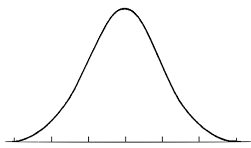
\includegraphics[width=.7\textwidth]{bell.png}
		\end{column}
		\begin{column}{.5\textwidth}
				$Pr(\eta = z) \sim$
		\end{column}
	\end{columns}
\alert{The symbol $\sim$ means ``is proportional to".}
\end{frame}

\begin{frame}
	\frametitle{quick check}
	\textbf{Example:} Linear Regression. 
	
	\textbf{Probabilistic model:}
	\begin{align*}
	y_i = \langle \bv{x}_i, \bs{\beta} \rangle+ \eta
	\end{align*}
	where the $\eta$ drawn from $N(0,\sigma^2)$ is \textbf{random Gaussian noise}.
	\vspace{.5em}
	
	\begin{center}
		\alert{If we knew $\bs{\beta}$ what is the \emph{maximum a posterior (MAP)} estimate for $y_i$ given observed data $\bv{x}_i$?}
	\end{center}
\end{frame}

\begin{frame}
	\frametitle{bayesian regression}
	\begin{center}
		\alert{How should be select $\bs{\beta}$ for our model?}
	\end{center}
		\textbf{Bayesian approach:} Use MAP estimate again! Now for parameter vector.
		
		 Choose $\bs{\beta}$ to  maximize:
		\begin{align*}
		\Pr(\bs{\beta} \mid \bv{X},\bv{y} )  = \frac{\Pr(\bv{X},\bv{y} \mid  \bs{\beta} ) \Pr(\bs{\beta} )  }{\Pr(\bv{X},\bv{y} )}.
		\end{align*}
		
		Assume all $\bs{\beta}$'s are equally likely, so we only care about $\Pr(\bv{X},\bv{y} \mid  \bs{\beta} )$  when maximizing.
		
		Choose $\bs{\beta}$ to  maximize:
		\begin{align*}
		\Pr(\bv{X},\bv{y}  \mid  \bs{\beta} ) \sim 
%		\prod_{i=1}^n e^{-(y_i - \langle \bv{x}_i, \bs{\beta} \rangle)^2/\sigma^2}
		\end{align*}
\end{frame}

\begin{frame}[t]
	\frametitle{bayesian regression}
	\begin{itemize}
		\item $y_i = \langle \bv{x}_i, \bs{\beta} \rangle+ \eta$
		\item where $p(\eta = z) \sim e^{-z^2/\sigma^2}$
		\vspace{1em}
		
		\begin{align*}
		\Pr(\bv{X},\bv{y}  \mid  \bs{\beta} ) \sim \hspace{10em}
		\end{align*}
	\end{itemize}
\end{frame}

\begin{frame}
	\frametitle{log likelihood}
	Easier to work with the \alert{\textbf{log likelihood}}:
	\begin{align*}
	\argmax_{\bs{\beta}}  \Pr(\bv{X},\bv{y}  \mid  \bs{\beta}) &=\argmax_{\bs{\beta}} \prod_{i=1}^n e^{-(y_i - \langle \bv{x}_i, \bs{\beta} \rangle)^2/\sigma^2} \\ 
	&= \argmax_{\bs{\beta}}\,\, \log\left(\prod_{i=1}^n e^{-(y_i - \langle \bv{x}_i, \bs{\beta} \rangle)^2/\sigma^2} \right)\\
	&= \argmax_{\bs{\beta}}  \sum_{i=1}^n -(y_i - \langle \bv{x}_i, \bs{\beta} \rangle)^2/\sigma^2\\
	&= \argmin_{\bs{\beta}}  \sum_{i=1}^n (y_i - \langle \bv{x}_i, \bs{\beta} \rangle)^2.
	\end{align*}
	
	Choose $\bs{\beta}$ to minimize $\sum_{i=1}^n (y_i - \langle \bv{x}_i, \bs{\beta} \rangle)^2 = \|\bv{y} - \bv{X}\bs{\beta}\|_2^2$!
	
	
	\alert{This is a completely different justification for squared loss.}
\end{frame}

\begin{frame}
	\frametitle{bayesian regression}
		If we had modeled our noise $\eta$ as Laplace noise, we would have found that minimizing $\|\bv{y} - \bv{X}\bs{\beta}\|_1$ was optimal.
		
		\vspace{1em}
		\begin{columns}
			\begin{column}{.5\textwidth}
				\hspace{2em}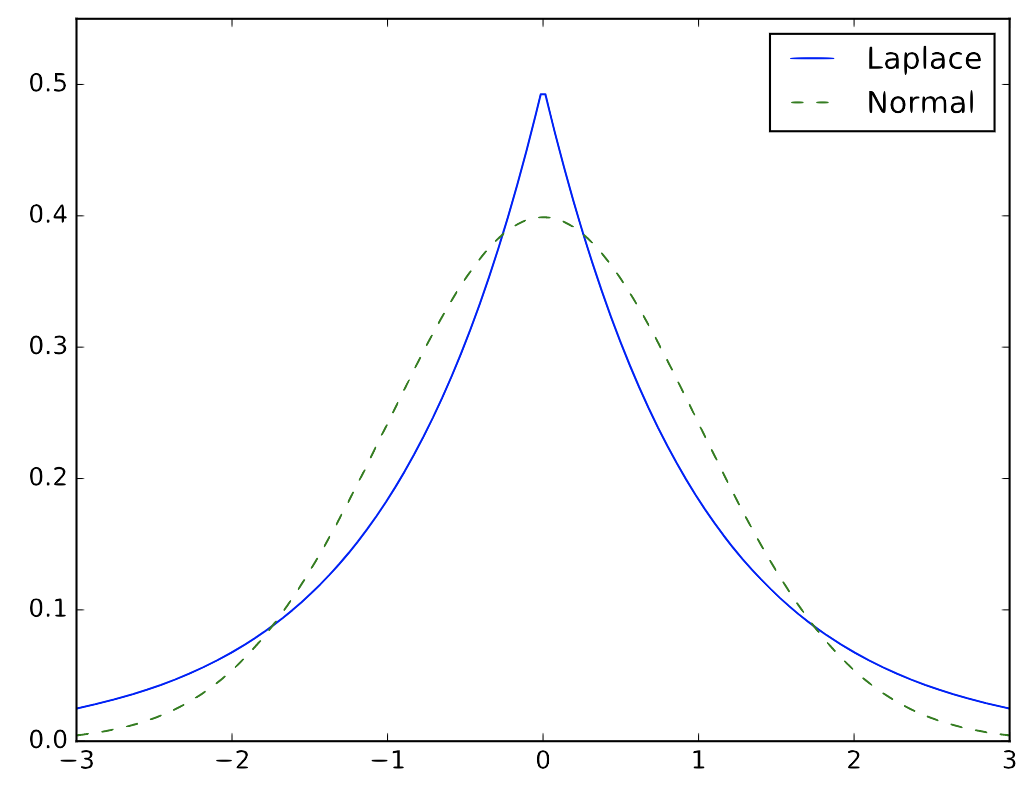
\includegraphics[width=.9\textwidth]{laplacen.png}
			\end{column}
			\begin{column}{.5\textwidth}
				$Pr(\eta = z) \sim$
			\end{column}
		\end{columns}
	
	Laplace noise has ``heavier tails'', meaning that it results in more outliers.
	
	\alert{This is a completely different justification for $\ell_1$ loss.}
\end{frame}

\begin{frame}
	\frametitle{bayesian regularization}
	\begin{center}
	\textbf{Recall goal is to maximize over $\bs{\beta}$:}
	\begin{align*}
		\Pr(\bs{\beta} \mid \bv{X},\bv{y} )  = \frac{\Pr(\bv{X},\bv{y} \mid  \bs{\beta} ) \Pr(\bs{\beta} )  }{\Pr(\bv{X},\bv{y} )}.
	\end{align*}
	\sout{assume all $\bs{\beta}$'s equally likely}	
	
	\textbf{Bayesian view:} Assume values in $\bs{\beta} = [\beta_1, \ldots, \beta_d]$ come from some distribution. 
	\end{center}

\begin{itemize}
	\item \textbf{Common model:} Each $\beta_i$ drawn from $N(0,\gamma^2)$, i.e. normally distributed, independent.
	\item Encodes a belief that we are unlikely to see models with very large coefficients. 
\end{itemize}
\end{frame}

\begin{frame}
	\frametitle{bayesian regularization}
	\textbf{Goal:}  choose $\bs{\beta}$ to maximize:
	\begin{align*}
		\Pr(\bs{\beta} \mid \bv{X},\bv{y} )  = \frac{\Pr(\bv{X},\bv{y} \mid  \bs{\beta} ) \Pr(\bs{\beta} )  }{\Pr(\bv{X},\bv{y} )} .
	\end{align*}
	\begin{itemize}
	\item We can still ignore the ``evidence'' term $\Pr(\bv{X},\bv{y})$ since it is a constant that does not depend on $\bs{\beta}$.
	\item $\Pr(\bs{\beta}) = \Pr({\beta}_1)\cdot  \Pr({\beta}_2)\cdot \ldots \cdot \Pr({\beta}_d)$
	\item $\Pr(\bs{\beta})  \sim $
	\end{itemize}
\end{frame}

\begin{frame}
	\frametitle{bayesian regularization}
	Easier to work with the {\textbf{log likelihood}}:
	\begin{align*}
	&\argmax_{\bs{\beta}}\Pr(\bv{X},\bv{y} \mid  \bs{\beta} ) \cdot \Pr(\bs{\beta} ) \\
	& = \argmax_{\bs{\beta}} \prod_{i=1}^n e^{-(y_i - \langle \bv{x}_i, \bs{\beta} \rangle)^2/\sigma^2} \cdot \prod_{i=1}^n e^{-(\beta_i)^2/\gamma^2} \\ 
	&= \argmax_{\bs{\beta}}  \sum_{i=1}^n -(y_i - \langle \bv{x}_i, \bs{\beta} \rangle)^2/\sigma^2 + \sum_{i=1}^d -(\beta_i)^2/\gamma^2\\
	&= \argmin_{\bs{\beta}}  \sum_{i=1}^n (y_i - \langle \bv{x}_i, \bs{\beta} \rangle)^2+ \frac{\sigma^2 }{\gamma^2}\sum_{i=1}^d (\beta_i)^2/\sigma^2.
	\end{align*}
	
	Choose $\bs{\beta}$ to minimize $\|\bv{y} - \bv{X}\bs{\beta}\|_2^2 + \frac{\sigma^2 }{\gamma^2}\|\bs{\beta}\|_2^2$.
	
	
	\alert{Completely different justification for ridge regularization!}
\end{frame}

\begin{frame}
	\frametitle{bayesian regularization}
	\textbf{Test your intuition:} What modeling assumption justifies LASSO regularization: $\min \|\bv{y} - \bv{X}\bs{\beta}\|_2^2 + \lambda\|\bs{\beta}\|_1$?
\end{frame}

\begin{frame}[standout]
	linear classification
\end{frame}

\begin{frame}
	\frametitle{motivating problem}
	\textbf{Breast Cancer Biopsy:} Determine if a breast lump in a patient is \emph{malignant} (cancerous) or \emph{benign} (safe). 
	\begin{itemize}
		\item Collect cells from lump using \emph{fine needle biopsy}.
		\item Stain and examine cells under microscope.
		\item Based on certain characteristics (shape, size, cohesion) determine if likely malignant or not).
	\end{itemize}
\begin{center}
	\includegraphics[width=.6\textwidth]{fna_labeled.png} \includegraphics[width=.4\textwidth]{cells.png}
\end{center}
\end{frame}

\begin{frame}
	\frametitle{motivating problem}
	\textbf{Demo:} \texttt{demo\_breast\_cancer.ipynb}
	
	\textbf{Data:} UCI machine learning repository
	\begin{center}
		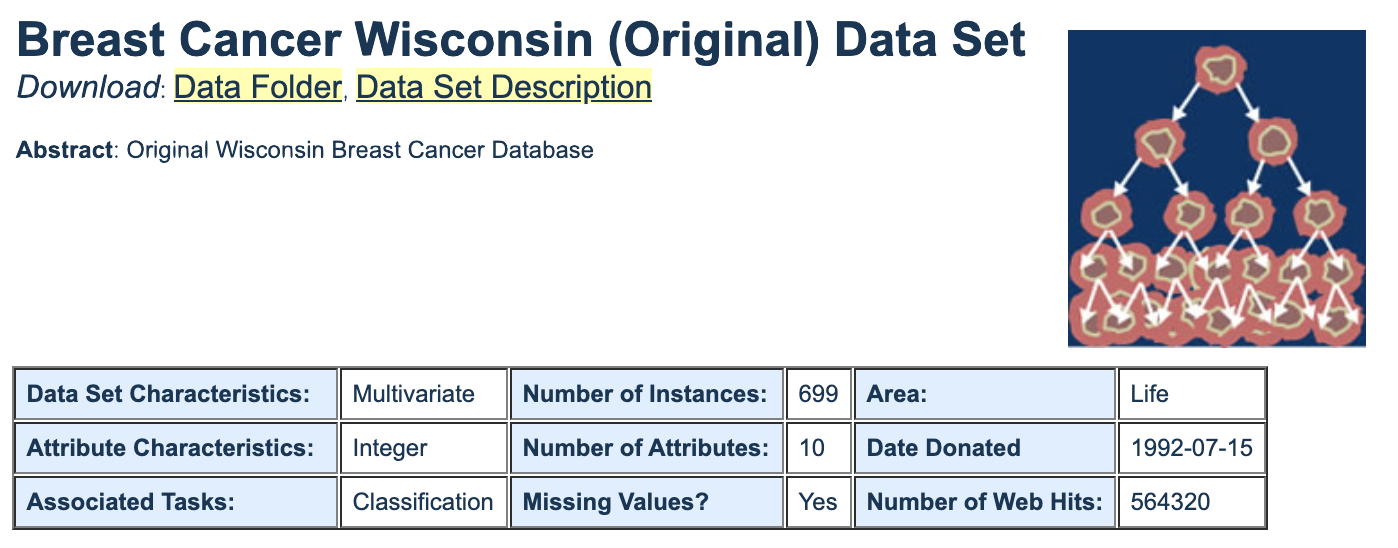
\includegraphics[width=.9\textwidth]{uci_cancer.png}
		
		\footnotesize{\url{https://archive.ics.uci.edu/ml/datasets/breast+cancer+wisconsin+(original)}}
	\end{center}

	\textbf{Features:} 10 numerical scores about cell characteristics (Clump Thickness, Uniformity, Marginal Adhesion, etc.)
	
\end{frame}

\begin{frame}
	\frametitle{motivating problem}
	\textbf{Data:} $(\bv{x}_1, y_1), \ldots, (\bv{x}_n, y_n)$. 
	
	$\bv{x}_i = [1,5,4\ldots, 2]$ contains score values. 
	
	Label $y_i\in \{0,1\}$ is $0$ if benign cells, $1$ if malignant cells.
	
	\textbf{Goal:} Based on scores (which would be collected manually, or even learned on their own using an ML algorithm) predict if a sample of cells is malignant or benign. 
	
	\textbf{Approach:}
	\begin{itemize}
		\item Naive Bayes Classifier can be extended to $\bv{x}$ with numerical values (instead of binary values as seen before).  Will see on homework.
		\item \textbf{Today:} Learn a different type of classifier.
	\end{itemize}
\end{frame}

\begin{frame}
	\frametitle{begin by plotting data}
	We pick two variables, \emph{Margin Adhesion} and \emph{Size Uniformity} and plot a scatter plot. Points with label 1 (malignant) are plotted in blue, those with label 2 (benign) are plotted in green.
	\begin{center}
		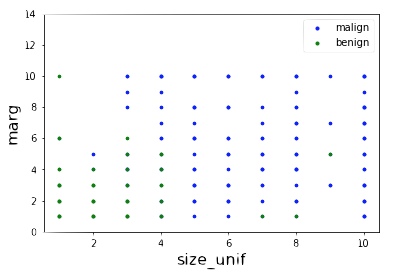
\includegraphics[width=.7\textwidth]{unjittered.png}
		
		\textbf{Lots of overlapping points! Hard to get a sense of the data.}
	\end{center}
\end{frame}

\begin{frame}
	\frametitle{plotting with jitter}
	\textbf{Simple + Useful Trick:} data \emph{jittering}. Add tiny random noise (using e.g. \texttt{np.random.randn}) to data to prevent overlap. 
	\begin{center}
		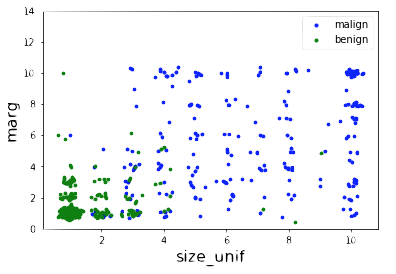
\includegraphics[width=.7\textwidth]{jittered.png}
		
		Noise is only for plotting. It is not added to the data for training, testing, etc. 
	\end{center}
\end{frame}

\begin{frame}
	\frametitle{plotting with jitter}
	\textbf{Simple + Useful Trick:} data \emph{jittering}. Add tiny random noise (using e.g. \texttt{np.random.randn}) to data to prevent overlap. 
	\begin{center}
		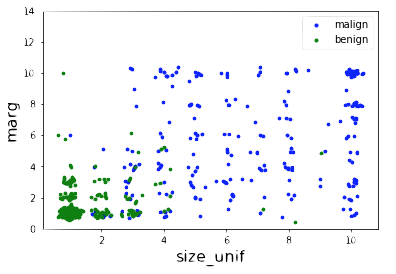
\includegraphics[width=.7\textwidth]{jittered.png}
		
		Noise is only for plotting. It is not added to the data for training, testing, etc. 
	\end{center}
\end{frame}

\begin{frame}
	\frametitle{brainstorming}
	\begin{center}
		Any ideas for possible \emph{classification rules} for this data?
		
		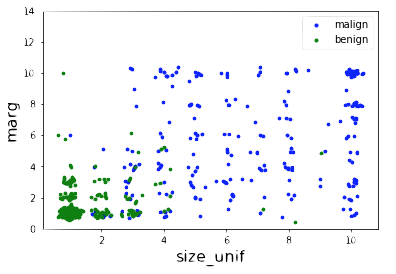
\includegraphics[width=.7\textwidth]{jittered.png}
		
	\end{center}
\end{frame}

\begin{frame}
	\frametitle{linear classifier}
	\begin{center}
		Given vector of predictors $\bv{x}_i \in \R^d$ (here $d = 2$) find a parameter vector $\bs{\beta} \in \R^d$ and threshold $\lambda$.
		\begin{itemize}
			\item Predict $y_i = 0$ if $\langle \bv{x}_i,\bs{\beta}\rangle \leq \lambda$.
			\item Predict $y_i = 1$ if $\langle \bv{x}_i,\bs{\beta}\rangle > \lambda$
		\end{itemize} 
		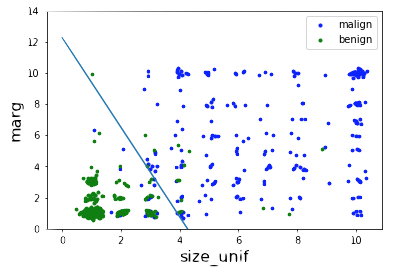
\includegraphics[width=.6\textwidth]{linear_classifier.png}
		
		\vspace{-.5em}
		Line has equation $\langle \bv{x}_i,\bs{\beta}\rangle  = \lambda$. 
	\end{center}
\end{frame}

\begin{frame}
	\frametitle{linear classifier}
	\begin{center}
	\textbf{Next class:} How do we find a good \alert{\textbf{linear separator}}?
	\end{center}
\end{frame}

\end{document} 








